%-----------------------------------------------------------------------------%
\chapter{\babTiga}
%-----------------------------------------------------------------------------%

Bab ini menjelaskan rancangan dan implementasi metode yang diusulkan, mulai dari penggunaan BERT sebagai \textit{feature extractor}, arsitektur model \textit{joint sentiment-topic} berbasis \textit{multitask learning}, peran \textit{autoencoder} dalam kompresi representasi, pengelompokan topik dengan \textit{Deep Embedded Clustering} (DEC), interpretasi model melalui analisis atribusi token, hingga evaluasi kualitas topik.

\begin{figure}[H]
    \centering
    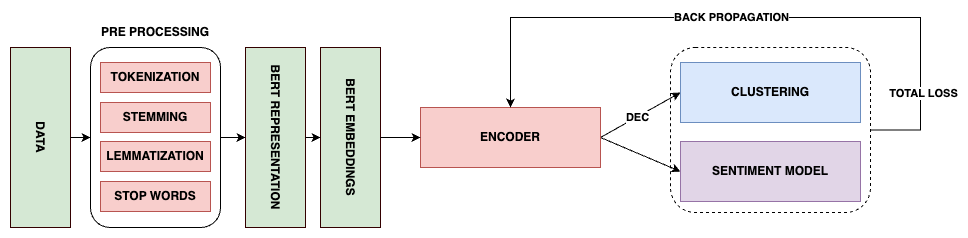
\includegraphics[width=0.9\textwidth]{assets/pics/MTL/FNN1.png}
    \caption{Alur metode analisis sentimen dan pendeteksian topik}
    \label{fig:alur_metode}
\end{figure}

%-----------------------------------------------------------------------------%
\section{\textit{Bidirectional Encoder Representations from Transformers}
(BERT) Sebagai Model Representasi Teks}
\label{sec:bert}
%-----------------------------------------------------------------------------%

Terdapat dua pendekatan utama dalam pemanfaatan model BERT, yaitu \textit{feature-based} dan \textit{fine-tuning}. Pada pendekatan \textit{feature-based}, BERT berfungsi sebagai \textit{feature extractor} tanpa mengubah parameter internalnya. Pada pendekatan \textit{fine-tuning}, lapisan keluaran khusus ditambahkan dan seluruh bobot dilatih ulang secara \textit{end-to-end}.

Pada penelitian ini, BERT digunakan melalui pendekatan \textit{feature-based} dengan bobot yang dibekukan sepenuhnya (\textit{frozen}). Representasi yang dihasilkan kemudian digunakan sebagai \textit{input} untuk \textit{autoencoder} dan pengelompokan topik menggunakan DEC. Contoh representasi teks yang dihasilkan BERT ditunjukkan pada Gambar~\ref{fig:bert_representasi}.

\begin{figure}[H]
    \centering
    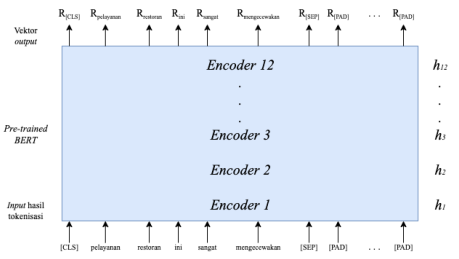
\includegraphics[width=0.7\textwidth]{assets/pics/BERT/BERT Rep-2.png}
    \caption{Representasi teks menggunakan BERT
             (\parencite{devlin2018bert}; telah diolah kembali).}
    \label{fig:bert_representasi}
\end{figure}

Sebagai ilustrasi, misalkan kalimat \textit{input} yang digunakan adalah \textit{``pelayanan restoran ini sangat mengecewakan''}. Proses pembentukan representasi teks oleh BERT dilakukan melalui beberapa tahapan berikut.

\begin{enumerate}
    \item \textbf{Tokenisasi.} Kalimat dipecah menjadi token menggunakan \textit{WordPiece tokenizer}, lalu ditambahkan token khusus \texttt{[CLS]} di awal dan \texttt{[SEP]} di akhir:
    \begin{center}
        \texttt{[[CLS], pelayanan, restoran, ini, sangat, mengecewakan, [SEP]]}.
    \end{center}

    \item \textbf{\textit{Padding}.} Token \texttt{[PAD]} ditambahkan agar panjang seluruh urutan seragam, misalnya hingga 10 token:
    \begin{center}
        \texttt{[[CLS], pelayanan, restoran, ini, sangat, mengecewakan, [SEP],
        [PAD], [PAD], [PAD]]}.
    \end{center}

    \item \textbf{\textit{Attention Mask}.} Dibuat \textit{attention mask} untuk membedakan token bermakna dengan token \textit{padding}. Token selain \texttt{[PAD]} diberi nilai 1 dan \texttt{[PAD]} diberi nilai 0:
    \begin{center}
        \textit{attention mask} $= [1, 1, 1, 1, 1, 1, 1, 0, 0, 0]$.
    \end{center}

    \item \textbf{\textit{Embedding}.} Token diubah menjadi representasi numerik melalui lapisan \textit{embedding}, yaitu hasil penjumlahan dari \textit{token embedding}, \textit{segment embedding}, dan \textit{position embedding}.

    \item \textbf{\textit{Encoding}.} Representasi diproses melalui beberapa lapisan \textit{encoder}, di mana setiap lapisan terdiri atas mekanisme \textit{multi-head self-attention}, \textit{feed-forward network}, koneksi residu, dan normalisasi.
\end{enumerate}

Model BERT \textit{pre-trained} yang digunakan terdiri atas 12 lapisan \textit{encoder} dengan ukuran \textit{hidden size} sebesar 768. Misalkan $t$ adalah panjang maksimum token dan $M$ adalah jumlah teks dalam \textit{dataset}, maka keluaran BERT berupa matriks berukuran $M \times t \times 768$. Pada penelitian ini, $t = 128$.

Pada tahap \textit{clustering}, representasi setiap teks harus berupa vektor, bukan matriks. Oleh karena itu, digunakan strategi ekstraksi token \texttt{[CLS]}, yang diletakkan di awal setiap urutan dan dilatih untuk merepresentasikan konteks global kalimat. Misalkan $\mathbf{H} = (h_{ij}) \in \mathbb{R}^{t \times 768}$ adalah matriks keluaran BERT untuk suatu teks, dengan $\mathbf{h}_i = (h_{i1}, h_{i2}, \ldots, h_{i,768})$ menyatakan representasi token ke-$i$. Vektor representasi dokumen $\mathbf{f}$ diperoleh dari baris pertama $\mathbf{H}$:

\begin{equation}
    \mathbf{f} = \mathbf{h}_1 \in \mathbb{R}^{768}
    \label{eq:cls_extraction}
\end{equation}

Vektor $\mathbf{f}$ ini selanjutnya digunakan sebagai \textit{input} untuk \textit{autoencoder} pada tahap berikutnya.

%-----------------------------------------------------------------------------%
\section{Model \textit{Joint Sentiment-Topic} Berbasis \textit{Multitask
Learning}}
%-----------------------------------------------------------------------------%

Penelitian ini mengusulkan model \textit{Joint Sentiment-Topic} berbasis \textit{Multitask Learning} untuk melakukan analisis sentimen dan pendeteksian topik secara bersamaan. Model ini dibangun di atas representasi BERT yang diproses melalui \textit{autoencoder} untuk menghasilkan representasi laten berdimensi rendah. Representasi laten tersebut digunakan bersama oleh dua \textit{head}, yaitu \textit{sentiment head} untuk klasifikasi sentimen dan \textit{clustering head} untuk pendeteksian topik melalui DEC. Pendekatan ini mengikuti skema \textit{hard parameter sharing}, di mana lapisan \textit{encoder} pada \textit{autoencoder} berfungsi sebagai jaringan bersama yang menerima gradien dari kedua tugas secara simultan.

Alur model terdiri atas tiga tahap. Pertama, representasi BERT berdimensi 768 diperoleh dari tahap ekstraksi fitur pada Bagian~\ref{sec:bert}. Kedua, representasi tersebut dikompresi oleh \textit{encoder} menjadi vektor laten $\mathbf{z}$ berdimensi lebih rendah. Ketiga, $\mathbf{z}$ digunakan secara bersamaan oleh kedua \textit{head} dalam satu kerangka optimasi bersama. Total \textit{loss} yang dioptimalkan selama pelatihan \textit{multitask} didefinisikan sebagai:

\begin{equation}
    \mathcal{L}_{\text{total}} = \gamma \cdot \mathcal{L}_{\text{KLD}}
    + \eta \cdot \mathcal{L}_{\text{CE}}
    \label{eq:total_loss}
\end{equation}

\noindent dengan $\gamma$ dan $\eta$ adalah koefisien bobot yang mengontrol kontribusi relatif antara \textit{loss} \textit{clustering} dan \textit{loss} klasifikasi sentimen.

%-----------------------------------------------------------------------------%
\section{Implementasi \textit{Autoencoder}}
%-----------------------------------------------------------------------------%

\textit{Autoencoder} umumnya sulit dilatih langsung karena rentan \textit{overfitting} dan sulit menemukan representasi yang stabil. Oleh karena itu, sebelum pelatihan \textit{multitask}, \textit{autoencoder} terlebih dahulu dilatih secara \textit{unsupervised} melalui proses \textit{pretraining} sebagai inisialisasi bobot awal.

Gambar~\ref{fig:autoencoder} menunjukkan ilustrasi arsitektur yang digunakan, mulai dari \textit{autoencoder} lengkap hingga komponen \textit{encoder} yang dipertahankan setelah \textit{pretraining}.

\begin{figure}[H]
    \centering
    \begin{subfigure}[b]{0.45\textwidth}
        \centering
        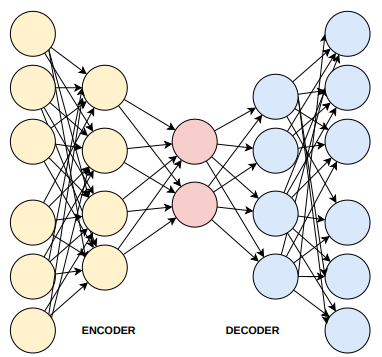
\includegraphics[height=5cm]{assets/pics/Autoencoder/Autoencoder0.png}
        \caption{\textit{Autoencoder} lengkap}
        \label{fig:autoencoder-full}
    \end{subfigure}
    \hfill
    \begin{subfigure}[b]{0.45\textwidth}
        \centering
        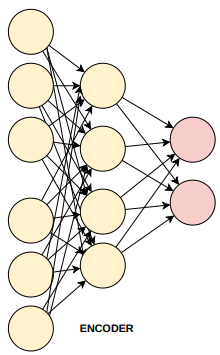
\includegraphics[height=5cm]{assets/pics/Autoencoder/Autoencoder1.png}
        \caption{\textit{Encoder}}
        \label{fig:encoder}
    \end{subfigure}
    \caption{Ilustrasi \textit{autoencoder} lengkap (kiri) dan komponen
    \textit{encoder} setelah \textit{decoder} dilepas (kanan).}
    \label{fig:autoencoder}
\end{figure}

Pada tahap \textit{pretraining}, jaringan dilatih untuk merekonstruksi kembali data \textit{input} dari representasi laten yang dihasilkan \textit{encoder}. Fungsi \textit{loss} yang digunakan adalah \textit{Mean Squared Error} (MSE) antara vektor \textit{input} asli dan hasil rekonstruksinya:

\begin{equation}
    \mathcal{L}_{\text{MSE}} = \frac{1}{N} \sum_{i=1}^{N}
    \left\| \mathbf{f}_i - \hat{\mathbf{f}}_i \right\|^2
    \label{eq:mse}
\end{equation}

\noindent dengan $N$ adalah jumlah total sampel, $\mathbf{f}_i$ adalah vektor representasi BERT ke-$i$, dan $\hat{\mathbf{f}}_i$ adalah hasil rekonstruksinya.

Fungsi aktivasi yang digunakan pada lapisan \textit{encoder} dan \textit{decoder} adalah \textit{Rectified Linear Unit} (ReLU), yang dipilih karena sesuai dengan distribusi representasi BERT yang dominan bernilai positif. 

Setelah \textit{pretraining} selesai, bobot \textit{encoder} digunakan sebagai inisialisasi untuk pelatihan \textit{multitask}. Pada tahap ini \textit{encoder} dipertahankan dan dioptimalkan bersama kedua \textit{head}, sedangkan \textit{decoder} tidak lagi digunakan. Representasi laten $\mathbf{z} = f_\theta(\mathbf{f})$ yang dihasilkan \textit{encoder} digunakan bersama oleh \textit{sentiment head} dan \textit{clustering head}.

%-----------------------------------------------------------------------------%
\section{Analisis Sentimen Menggunakan \textit{Sentiment Head}}
%-----------------------------------------------------------------------------%

Vektor laten $\mathbf{z} \in \mathbb{R}^{256}$ yang dihasilkan \textit{encoder} diteruskan ke \textit{sentiment head} untuk diklasifikasikan ke salah satu dari dua kelas sentimen. Arsitektur \textit{sentiment head} terdiri atas tiga lapisan linear bertingkat dengan dimensi $256 \to 256 \to 32 \to 2$. Setiap lapisan tersembunyi dilengkapi dengan \textit{batch normalization}, fungsi aktivasi \textit{Gaussian Error Linear Unit} (GELU), dan \textit{dropout} dengan probabilitas $p = 0{,}5$. Lapisan keluaran berdimensi dua diikuti fungsi \textit{softmax} untuk menghasilkan distribusi probabilitas antarkelas. Arsitektur lengkapnya diilustrasikan pada Gambar~\ref{fig:sentiment_head} berikut.

\begin{figure}[H]
\centering
\begin{tikzpicture}[
    node distance=0.4cm and 0.7cm,
    box/.style={rectangle, rounded corners=4pt, draw, align=center,
                font=\small, minimum height=1cm, minimum width=2cm},
    inbox/.style={box,  fill=blue!8,    draw=blue!40},
    fcbox/.style={box,  fill=purple!12, draw=purple!50},
    bnbox/.style={box,  fill=gray!12,   draw=gray!50},
    actbox/.style={box, fill=orange!15, draw=orange!50},
    dropbox/.style={box,fill=cyan!12,   draw=cyan!50},
    outbox/.style={box, fill=green!8,   draw=green!40},
    arrow/.style={-{Stealth[length=5pt]}, thick}
]

\node[inbox] (z) {$\mathbf{z} \in \mathbb{R}^{256}$};

\node[fcbox,   right=of z]    (fc1)   {\textit{Linear}\\{\scriptsize$256 \to 256$}};
\node[bnbox,   right=of fc1]  (bn1)   {\textit{BatchNorm}\\{\scriptsize$256$}};
\node[actbox,  right=of bn1]  (gelu1) {GELU};
\node[dropbox, right=of gelu1](drop1) {\textit{Dropout}\\{\scriptsize$p=0{,}5$}};

\node[fcbox,   below=1.2cm of fc1]   (fc2)   {\textit{Linear}\\{\scriptsize$256 \to 32$}};
\node[bnbox,   right=of fc2]         (bn2)   {\textit{BatchNorm}\\{\scriptsize$32$}};
\node[actbox,  right=of bn2]         (gelu2) {GELU};
\node[dropbox, right=of gelu2]       (drop2) {\textit{Dropout}\\{\scriptsize$p=0{,}5$}};

\node[fcbox,  below=1.2cm of fc2]    (fc3)     {\textit{Linear}\\{\scriptsize$32 \to 2$}};
\node[outbox, right=2.5cm of fc3]    (softmax) {\textit{Softmax}\\{\scriptsize pos / neg}};

\draw[arrow] (z)     -- (fc1);
\draw[arrow] (fc1)   -- (bn1);
\draw[arrow] (bn1)   -- (gelu1);
\draw[arrow] (gelu1) -- (drop1);
\draw[arrow] (drop1.south) -- ++(0,-0.35) -| (fc2.north);
\draw[arrow] (fc2)   -- (bn2);
\draw[arrow] (bn2)   -- (gelu2);
\draw[arrow] (gelu2) -- (drop2);
\draw[arrow] (drop2.south) -- ++(0,-0.35) -| (fc3.north);
\draw[arrow] (fc3)   -- (softmax);

\end{tikzpicture}
\caption{Arsitektur \textit{sentiment head}.}
\label{fig:sentiment_head}
\end{figure}

Proses klasifikasi dirumuskan sebagai:

\begin{equation}
    \hat{\mathbf{y}} = \text{softmax}\!\left(\mathbf{W}_c \mathbf{z}
    + \mathbf{b}_c\right)
    \label{eq:sentiment_cls}
\end{equation}

\noindent dengan $\mathbf{W}_c$ dan $\mathbf{b}_c$ masing-masing adalah bobot dan bias pada lapisan keluaran. Fungsi \textit{softmax} mengubah nilai logit menjadi distribusi probabilitas, di mana setiap elemen $\hat{y}_i \in [0, 1]$ dan $\sum_i \hat{y}_i = 1$.

Selama pelatihan, prediksi $\hat{\mathbf{y}}$ dibandingkan dengan label sebenarnya $\mathbf{y}$ menggunakan fungsi \textit{loss Categorical Cross-Entropy}:

\begin{equation}
    \mathcal{L}_{\text{CE}} = -\sum_{i=1}^{N} \sum_{j=1}^{2}
    y_{ij} \log \hat{y}_{ij}
    \label{eq:ce_loss}
\end{equation}

\noindent dengan $N$ adalah jumlah sampel, $y_{ij}$ adalah label aktual dalam bentuk \textit{one-hot} bernilai 1 jika sampel ke-$i$ termasuk kelas ke-$j$ dan 0 jika tidak, serta $\hat{y}_{ij}$ adalah probabilitas prediksi model. $\mathcal{L}_{\text{CE}}$ ini menjadi salah satu komponen dari total \textit{loss} pada Persamaan~\eqref{eq:total_loss}.

%-----------------------------------------------------------------------------%
\section{\textit{Deep Embedded Clustering} (DEC) dan \textit{Clustering Head}}
%-----------------------------------------------------------------------------%

Selain \textit{sentiment head}, vektor laten $\mathbf{z}$ yang sama diteruskan ke \textit{clustering head} untuk pendeteksian topik. \textit{Clustering head} diimplementasikan menggunakan DEC, yang bertujuan memperbarui representasi laten dan menyesuaikan posisi \textit{centroid} agar sesuai dengan struktur distribusi data pada ruang laten \parencite{xie2016unsupervised}. Berbeda dengan \textit{hard assignment} yang menetapkan setiap sampel ke satu klaster, DEC menggunakan distribusi probabilistik sehingga setiap sampel memiliki derajat keanggotaan terhadap seluruh klaster. Arsitektur \textit{clustering head} diilustrasikan pada Gambar~\ref{fig:clustering_head} berikut.

\begin{figure}[H]
\centering
\resizebox{\textwidth}{!}{%
\begin{tikzpicture}[
    node distance=0.4cm and 0.7cm,
    box/.style={rectangle, rounded corners=4pt, draw, align=center,
                font=\small, minimum height=1cm, minimum width=2.6cm},
    inbox/.style={box,  fill=blue!8,    draw=blue!40},
    cbox/.style={box,   fill=teal!12,   draw=teal!50},
    distbox/.style={box,fill=yellow!15, draw=yellow!50},
    targbox/.style={box,fill=orange!12, draw=orange!50},
    outbox/.style={box, fill=green!8,   draw=green!40},
    arrow/.style={-{Stealth[length=5pt]}, thick}
]

\node[inbox] (z) {$\mathbf{z} \in \mathbb{R}^{256}$};

\node[cbox,    right=of z]    (cent)
    {\textit{Clustering Layer}\\
     {\scriptsize$K$ \textit{centroid}}\\
     {\scriptsize$\boldsymbol{\mu}_j \in \mathbb{R}^{256}$}};

\node[distbox, right=of cent] (soft)
    {\textit{Soft Assignment}\\
     {\scriptsize Student's $t$}\\
     {\scriptsize$q_{ij}$}};

\node[targbox, right=of soft] (target)
    {\textit{Target Distribution}\\
     {\scriptsize dipertajam}\\
     {\scriptsize$p_{ij}$}};

\node[outbox,  right=of target] (label)
    {Label Topik\\
     {\scriptsize$\arg\max_j\, q_{ij}$}};

\draw[arrow] (z)      -- (cent);
\draw[arrow] (cent)   -- (soft);
\draw[arrow] (soft)   -- (target);
\draw[arrow] (target) -- (label);

\end{tikzpicture}%
}
\caption{Arsitektur \textit{clustering head} berbasis DEC.}
\label{fig:clustering_head}
\end{figure}

Proses DEC dimulai dengan inisialisasi \textit{centroid} menggunakan K-Means pada representasi laten awal hasil \textit{pretraining autoencoder}. Selanjutnya, distribusi \textit{soft assignment} $q_{ij}$ untuk setiap data $\mathbf{z}_i$ terhadap \textit{centroid} $\boldsymbol{\mu}_j$ dihitung menggunakan distribusi Student's $t$:

\begin{equation}
    q_{ij} = \frac{\left(1 + \left\|\mathbf{z}_i -
    \boldsymbol{\mu}_j\right\|^2\right)^{-1}}
    {\displaystyle\sum_{j'=1}^{K}\left(1 + \left\|\mathbf{z}_i -
    \boldsymbol{\mu}_{j'}\right\|^2\right)^{-1}}
    \label{eq:soft_assign}
\end{equation}

\noindent dengan $q_{ij}$ menyatakan probabilitas sampel $i$ termasuk klaster $j$, dan $K$ adalah jumlah klaster.

Selanjutnya, DEC mendefinisikan distribusi target $p_{ij}$ yang lebih 
terkonsentrasi (\textit{sharpened}) agar setiap sampel lebih condong ke 
satu klaster. Misalkan $f_j = \sum_{i} q_{ij}$ adalah frekuensi 
\textit{soft} klaster $j$, maka:

\begin{equation}
    p_{ij} = \frac{q_{ij}^2 \,/\, f_j}
    {\displaystyle\sum_{j'=1}^{K} q_{ij'}^2 \,/\, f_{j'}}
    \label{eq:target_dist}
\end{equation}

Pembagian dengan $f_j$ mencegah klaster besar mendominasi proses 
optimasi, sedangkan kuadrat pada $q_{ij}$ membuat distribusi lebih 
terkonsentrasi pada satu klaster. Optimasi dilakukan dengan meminimalkan 
\textit{Kullback-Leibler Divergence} antara distribusi target $P$ dan 
distribusi \textit{soft assignment} $Q$:

\begin{equation}
    \mathcal{L}_{\text{KLD}} = \sum_{i}\sum_{j}
    p_{ij} \log\frac{p_{ij}}{q_{ij}}
    \label{eq:kld}
\end{equation}

\noindent $\mathcal{L}_{\text{KLD}}$ digunakan sebagai dasar untuk memperbarui parameter \textit{encoder} dan posisi \textit{centroid} menggunakan optimizer Adam secara iteratif. Pada setiap \textit{update interval}, label klaster hasil iterasi sebelumnya akan dibandingkan dengan label terbaru. Proses pelatihan dihentikan apabila perubahan label klaster ($\Delta_{\text{label}}$) berada di bawah batas toleransi $\tau$. Prosedur lengkap metode ini disajikan pada Tabel~\ref{tab:alg_dec} berikut.

\begin{table}[H]
\centering
\caption{Algoritma \textit{Deep Embedded Clustering} (DEC)}
\label{tab:alg_dec}
\begin{tabular}{p{0.05\textwidth} p{0.85\textwidth}}
\hline
\multicolumn{2}{l}{\textbf{Algoritma} \textit{Deep Embedded Clustering} (DEC)} \\
\hline
\multicolumn{2}{l}{\textbf{INPUT} \hspace{1.2em}
    Himpunan vektor data $\{\mathbf{f}_i\}_{i=1}^{N} \in \mathbb{R}^{768}$;
    jumlah klaster $K$;} \\
\multicolumn{2}{l}{\hspace{4.7em}
    \textit{batch size} $b$; batas toleransi konvergensi $\tau$;} \\
\multicolumn{2}{l}{\hspace{4.7em}
    parameter bobot \textit{loss} $\gamma$, $\eta$;
    jumlah iterasi maksimum $T_{\max}$} \\[2pt]
\multicolumn{2}{l}{\textbf{OUTPUT}
    Representasi laten $\{\mathbf{z}_i\}$;
    label klaster $\{y_{\text{cluster}}\}$;
    label sentimen $\{y_{\text{sentiment}}\}$} \\
\hline
1. & Latih \textit{autoencoder} dengan meminimalkan MSE: \\
   & \hspace{1.5em}
     $\mathcal{L}_{\text{MSE}} = \dfrac{1}{N}\displaystyle\sum_{i=1}^{N}
     \|\mathbf{f}_i - \hat{\mathbf{f}}_i\|^2$ \\[6pt]
2. & Ambil bagian \textit{encoder} untuk memperoleh representasi laten
     $\mathbf{z}_i = f_\theta(\mathbf{f}_i)$ \\[3pt]
3. & Inisialisasi \textit{centroid} awal $\{\boldsymbol{\mu}_j\}_{j=1}^{K}$
     menggunakan K-Means pada $\{\mathbf{z}_i\}$ \\[3pt]
4. & \textbf{FOR} iter $= 1$ hingga $T_{\max}$ \\[3pt]
   & \hspace{1em} 4.1 \hspace{0.5em}
     Simpan label klaster sebelumnya $y_{\text{prev}}$ \\[3pt]
   & \hspace{1em} 4.2 \hspace{0.5em}
     Proyeksikan data ke ruang laten: $\mathbf{z}_i = f_\theta(\mathbf{f}_i)$ \\[3pt]
   & \hspace{1em} 4.3 \hspace{0.5em}
     Hitung \textit{soft assignment} $q_{ij}$ menggunakan distribusi
     Student's $t$ \\[3pt]
   & \hspace{1em} 4.4 \hspace{0.5em}
     Hitung distribusi target $p_{ij}$ berdasarkan $q_{ij}$ \\[3pt]
   & \hspace{1em} 4.5 \hspace{0.5em}
     Hitung keluaran sentimen
     $\hat{\mathbf{y}} = \text{softmax}(\mathbf{W}_c\mathbf{z} +
     \mathbf{b}_c)$ \\[3pt]
   & \hspace{1em} 4.6 \hspace{0.5em}
     Perbarui parameter model dengan meminimalkan \textit{joint loss}: \\
   & \hspace{3em}
     $\mathcal{L}_{\text{total}} = \gamma \cdot \mathcal{L}_{\text{KLD}}(P,
     Q) + \eta \cdot \mathcal{L}_{\text{CE}}(\mathbf{y}, \hat{\mathbf{y}})$ \\[3pt]
   & \hspace{1em} 4.7 \hspace{0.5em}
     Jika $\Delta_{\text{label}} < \tau$, hentikan pelatihan \\[3pt]
5. & \textbf{END FOR} \\[3pt]
6. & Simpan bobot terbaik model berdasarkan metrik validasi \\
\hline
\multicolumn{2}{l}{\textbf{OUTPUT:}
    Representasi laten $\{\mathbf{z}_i\}$,
    label klaster $\{y_{\text{cluster}}\}$,
    dan label sentimen $\{y_{\text{sentiment}}\}$} \\
\hline
\end{tabular}
\end{table}

%-----------------------------------------------------------------------------%
\section{Pelatihan \textit{Joint} dengan \textit{Multitask Loss}}
%-----------------------------------------------------------------------------%

Total \textit{loss} yang dioptimalkan adalah Persamaan~\eqref{eq:total_loss}, yaitu kombinasi berbobot antara $\mathcal{L}_{\text{KLD}}$ dari \textit{clustering head} dan $\mathcal{L}_{\text{CE}}$ dari \textit{sentiment head}. Koefisien $\gamma$ mengontrol kontribusi informasi pengelompokan, sedangkan $\eta$ mengontrol kontribusi informasi sentimen.

Gradien dari $\mathcal{L}_{\text{KLD}}$ mengarahkan \textit{encoder} untuk membentuk representasi yang terstruktur berdasarkan klaster, sementara gradien dari $\mathcal{L}_{\text{CE}}$ mengarahkan representasi laten agar lebih mampu membedakan label sentimen.

Nilai $\gamma$ dan $\eta$ ditentukan melalui pencarian \textit{hyperparameter} pada data validasi. Jika $\gamma \gg \eta$, model cenderung mengutamakan struktur klaster; sebaliknya jika $\eta \gg \gamma$, representasi laten lebih diarahkan oleh informasi sentimen.

%-----------------------------------------------------------------------------%
\section{Interpretasi Model dengan Analisis Atribusi Token}
%-----------------------------------------------------------------------------%

Penelitian ini menerapkan dua metode interpretasi \textit{post-hoc}, yaitu \textit{occlusion-based token attribution} pada level token dan \textit{Integrated Gradients} pada level dimensi \textit{embedding}. Keduanya diterapkan setelah pelatihan selesai menggunakan bobot model terbaik.

%-----------------------------------------------------------------------------%
\subsection{Implementasi \textit{Occlusion-based Token Attribution} dan
Agregasi per Klaster}
%-----------------------------------------------------------------------------%

Teks \textit{input} $\mathbf{x}$ diproses oleh BERT untuk menghasilkan representasi \texttt{[CLS]}, yang kemudian diteruskan ke \textit{sentiment head} guna memperoleh probabilitas \textit{baseline} $f_c(\mathbf{x})$ untuk kelas $c$. Berikutnya, setiap token $x_i$ dalam teks, kecuali token-token spesial \texttt{[CLS]}, \texttt{[SEP]}, dan \texttt{[PAD]}, digantikan dengan \texttt{[MASK]} sehingga menghasilkan varian teks $\mathbf{x}_{\setminus i}$. Varian tersebut kemudian diproses kembali melalui BERT dan \textit{sentiment head} untuk memperoleh probabilitas yang diperbarui, $f_c(\mathbf{x}_{\setminus i})$. Skor atribusi token $x_i$ terhadap kelas $c$ selanjutnya dihitung dengan:

\begin{equation}
    \text{Attr}(x_i, c) = f_c(\mathbf{x}) - f_c(\mathbf{x}_{\setminus i})
    \label{eq:occlusion_bab3}
\end{equation}

Nilai positif mengindikasikan bahwa token $x_i$ berkontribusi terhadap prediksi kelas $c$, nilai negatif mengindikasikan kontribusi yang berlawanan arah, sedangkan nilai yang mendekati nol mengindikasikan bahwa token tidak memberikan pengaruh yang berarti.

Skor atribusi kemudian diagregasi per klaster untuk melihat pola linguistik pada level topik. Misalkan $\mathcal{C}_k = \{i : z_i = k\}$ adalah himpunan sampel pada klaster $k$, dengan $z_i$ adalah label klaster sampel ke-$i$. Skor atribusi rata-rata token $w$ pada klaster $k$ didefinisikan sebagai:

\begin{equation}
    \overline{\text{Attr}}(w, k, c) =
    \frac{1}{|\mathcal{C}_k|}
    \sum_{i \in \mathcal{C}_k} \text{Attr}(x_i^{(w)}, c)
    \label{eq:cluster_attr}
\end{equation}

\noindent dengan $x_i^{(w)}$ merujuk pada posisi token $w$ dalam sampel ke-$i$ dan $|\mathcal{C}_k|$ adalah jumlah sampel dalam klaster $k$. Hanya token yang muncul pada minimal dua sampel dalam klaster yang sama yang diikutsertakan, yaitu:

\begin{equation}
    \mathcal{V}_k = \left\{ w \;\middle|\;
    \sum_{i \in \mathcal{C}_k} \mathbf{1}[w \in \mathbf{x}_i]
    \geq 2 \right\}
    \label{eq:vocab_filter}
\end{equation}

Token dalam $\mathcal{V}_k$ diurutkan berdasarkan nilai absolut skor atribusi rata-rata untuk memperoleh daftar $R$ token paling berpengaruh pada klaster $k$:

\begin{equation}
    \text{TopTokens}(k, c) =
    \underset{w \in \mathcal{V}_k}{\text{arg top-}R} \;
    \left| \overline{\text{Attr}}(w, k, c) \right|
    \label{eq:top_tokens}
\end{equation}

Dalam implementasinya, kosakata yang dievaluasi dibatasi pada \textit{top-N} kata berdasarkan TF-IDF per klaster, sehingga skor atribusi hanya dihitung untuk kata-kata yang khas di klaster tersebut.

%-----------------------------------------------------------------------------%
\subsection{Implementasi \textit{Integrated Gradients}}
%-----------------------------------------------------------------------------%

\textit{Integrated Gradients} diterapkan pada level dimensi \textit{embedding} untuk mengidentifikasi dimensi yang paling berpengaruh terhadap prediksi sentimen. \textit{Baseline} yang digunakan adalah vektor nol $\mathbf{x'} = \mathbf{0} \in \mathbb{R}^d$, dengan jumlah langkah interpolasi $m = 50$ sebagaimana direkomendasikan oleh \textcite{sundararajan2017axiomatic}. Atribusi IG untuk setiap dimensi \textit{embedding} diaproksimasi menggunakan \textit{Riemann sum}:

\begin{equation}
    \text{IG}_i(\mathbf{x}) \approx (x_i - x'_i) \times
    \sum_{k=1}^{m}
    \frac{\partial f\!\left(\mathbf{x'} + \frac{k}{m}
    (\mathbf{x} - \mathbf{x'})\right)}{\partial x_i} \times
    \frac{1}{m}
    \label{eq:ig_approx_bab3}
\end{equation}

\noindent dengan $x_i$ adalah nilai dimensi ke-$i$ dari \textit{embedding} \textit{input}, $x'_i$ adalah nilai \textit{baseline} pada dimensi yang sama, dan $\frac{\partial f}{\partial x_i}$ adalah gradien prediksi model terhadap dimensi ke-$i$. Atribusi IG kemudian diagregasi per klaster:

\begin{equation}
    \overline{\text{IG}}_i(k) = \frac{1}{|\mathcal{C}_k|}
    \sum_{j \in \mathcal{C}_k} \left| \text{IG}_i(\mathbf{x}_j)
    \right|
    \label{eq:ig_cluster}
\end{equation}

\noindent dengan $\overline{\text{IG}}_i(k)$ adalah rata-rata nilai absolut atribusi IG dimensi ke-$i$ pada klaster $k$, dan $\mathbf{x}_j$ adalah \textit{embedding} sampel ke-$j$ dalam klaster $k$. Hasil agregasi ini divisualisasikan dalam bentuk \textit{heatmap} untuk memudahkan perbandingan antarkelas.

%-----------------------------------------------------------------------------%
\section{Evaluasi Topik}
\label{sec:topic_eval}
%-----------------------------------------------------------------------------%

Evaluasi kualitas topik dilakukan menggunakan tiga metrik kuantitatif, yaitu \textit{topic coherence}, \textit{topic diversity}, dan \textit{topic coverage}. Ketiga metrik dihitung langsung dari teks asli dan hasil pengelompokan klaster tanpa bergantung pada model eksternal.

%-----------------------------------------------------------------------------%
\subsection{\textit{Topic Coherence} Berbasis NPMI}
\label{sec:coherence}
%-----------------------------------------------------------------------------%

\textit{Topic coherence} mengukur sejauh mana kata-kata teratas suatu topik sering muncul bersama dalam korpus. Metrik yang digunakan adalah \textit{Normalized Pointwise Mutual Information} (NPMI) untuk mengukur ko-okurrens antar pasangan kata dalam klaster yang sama.

Misalkan $\mathcal{D}_k$ adalah himpunan teks dalam klaster $k$ dan $\{w_1, w_2, \ldots, w_N\}$ adalah $N$ kata teratas dari klaster tersebut berdasarkan frekuensi kemunculan setelah pemfilteran \textit{stop words}. Untuk setiap pasangan kata $(w_i, w_j)$ dengan $i < j$, probabilitas kemunculan masing-masing kata dan ko-okurrensnya didefinisikan sebagai:

\begin{align}
    p(w_i) &= \frac{|\{d \in \mathcal{D}_k : w_i \in d\}|}{|\mathcal{D}_k|}, \\[4pt]
    p(w_j) &= \frac{|\{d \in \mathcal{D}_k : w_j \in d\}|}{|\mathcal{D}_k|}, \\[4pt]
    p(w_i, w_j) &= \frac{|\{d \in \mathcal{D}_k :
        w_i \in d \text{ dan } w_j \in d\}|}{|\mathcal{D}_k|}.
\end{align}

Nilai \textit{Pointwise Mutual Information} (PMI) antara dua kata dihitung sebagai:

\begin{equation}
    \mathrm{PMI}(w_i, w_j) = \log \frac{p(w_i, w_j) + \varepsilon}
    {p(w_i) \cdot p(w_j) + \varepsilon}
    \label{eq:pmi}
\end{equation}

\noindent dengan $\varepsilon = 10^{-10}$ untuk menghindari pembagian dengan nol. Selanjutnya, PMI dinormalisasi menggunakan probabilitas ko-okurrens sebagai pembagi:

\begin{equation}
    \mathrm{NPMI}(w_i, w_j) = \frac{\mathrm{PMI}(w_i, w_j)}
    {-\log\bigl(p(w_i, w_j) + \varepsilon\bigr)}
    \label{eq:npmi}
\end{equation}

Nilai NPMI berada pada rentang $[-1, 1]$: mendekati $1$ berarti ko-okurrens tinggi, $0$ berarti independen, dan negatif berarti kata-kata jarang muncul bersama. Skor \textit{topic coherence} untuk klaster $k$ adalah rata-rata NPMI atas semua pasangan kata teratas:

\begin{equation}
    \mathrm{TC}_k = \frac{1}{\binom{N}{2}} \sum_{j=2}^{N} \sum_{i=1}^{j-1}
        \mathrm{NPMI}(w_i, w_j)
    \label{eq:tc_cluster}
\end{equation}

Skor koherensi keseluruhan diperoleh dengan merata-ratakan $\mathrm{TC}_k$ di seluruh klaster:

\begin{equation}
    \overline{\mathrm{TC}} = \frac{1}{K} \sum_{k=1}^{K} \mathrm{TC}_k
    \label{eq:tc_mean}
\end{equation}

Metrik ini hanya dihitung untuk klaster dengan setidaknya dua kata teratas yang unik; klaster yang tidak memenuhi syarat diberi nilai koherensi $0$.

%-----------------------------------------------------------------------------%
\subsection{\textit{Topic Diversity}}
\label{sec:diversity}
%-----------------------------------------------------------------------------%

\textit{Topic diversity} mengukur seberapa berbeda kosakata antarkelas. Misalkan $\mathcal{W}_k$ adalah himpunan $N$ kata teratas dari klaster $k$, himpunan kata unik di seluruh klaster $\mathcal{U} = \bigcup_{k=1}^{K} \mathcal{W}_k$, dan total kata termasuk duplikat adalah $\sum_{k=1}^{K} |\mathcal{W}_k|$. \textit{Topic diversity} didefinisikan sebagai:

\begin{equation}
    \mathrm{TD} = \frac{|\mathcal{U}|}{\displaystyle\sum_{k=1}^{K}
    |\mathcal{W}_k|}
    \label{eq:td}
\end{equation}

Nilai $\mathrm{TD} = 1$ berarti seluruh kata teratas antarkelas unik, sedangkan nilai rendah menunjukkan banyak tumpang tindih kosakata.